
\documentclass{article} % For LaTeX2e
\usepackage{iclr2025_conference,times}
\usepackage{graphicx}

% Optional math commands from https://github.com/goodfeli/dlbook_notation.
%%%%% NEW MATH DEFINITIONS %%%%%

\usepackage{amsmath,amsfonts,bm}

% Mark sections of captions for referring to divisions of figures
\newcommand{\figleft}{{\em (Left)}}
\newcommand{\figcenter}{{\em (Center)}}
\newcommand{\figright}{{\em (Right)}}
\newcommand{\figtop}{{\em (Top)}}
\newcommand{\figbottom}{{\em (Bottom)}}
\newcommand{\captiona}{{\em (a)}}
\newcommand{\captionb}{{\em (b)}}
\newcommand{\captionc}{{\em (c)}}
\newcommand{\captiond}{{\em (d)}}

% Highlight a newly defined term
\newcommand{\newterm}[1]{{\bf #1}}


% Figure reference, lower-case.
\def\figref#1{figure~\ref{#1}}
% Figure reference, capital. For start of sentence
\def\Figref#1{Figure~\ref{#1}}
\def\twofigref#1#2{figures \ref{#1} and \ref{#2}}
\def\quadfigref#1#2#3#4{figures \ref{#1}, \ref{#2}, \ref{#3} and \ref{#4}}
% Section reference, lower-case.
\def\secref#1{section~\ref{#1}}
% Section reference, capital.
\def\Secref#1{Section~\ref{#1}}
% Reference to two sections.
\def\twosecrefs#1#2{sections \ref{#1} and \ref{#2}}
% Reference to three sections.
\def\secrefs#1#2#3{sections \ref{#1}, \ref{#2} and \ref{#3}}
% Reference to an equation, lower-case.
\def\eqref#1{equation~\ref{#1}}
% Reference to an equation, upper case
\def\Eqref#1{Equation~\ref{#1}}
% A raw reference to an equation---avoid using if possible
\def\plaineqref#1{\ref{#1}}
% Reference to a chapter, lower-case.
\def\chapref#1{chapter~\ref{#1}}
% Reference to an equation, upper case.
\def\Chapref#1{Chapter~\ref{#1}}
% Reference to a range of chapters
\def\rangechapref#1#2{chapters\ref{#1}--\ref{#2}}
% Reference to an algorithm, lower-case.
\def\algref#1{algorithm~\ref{#1}}
% Reference to an algorithm, upper case.
\def\Algref#1{Algorithm~\ref{#1}}
\def\twoalgref#1#2{algorithms \ref{#1} and \ref{#2}}
\def\Twoalgref#1#2{Algorithms \ref{#1} and \ref{#2}}
% Reference to a part, lower case
\def\partref#1{part~\ref{#1}}
% Reference to a part, upper case
\def\Partref#1{Part~\ref{#1}}
\def\twopartref#1#2{parts \ref{#1} and \ref{#2}}

\def\ceil#1{\lceil #1 \rceil}
\def\floor#1{\lfloor #1 \rfloor}
\def\1{\bm{1}}
\newcommand{\train}{\mathcal{D}}
\newcommand{\valid}{\mathcal{D_{\mathrm{valid}}}}
\newcommand{\test}{\mathcal{D_{\mathrm{test}}}}

\def\eps{{\epsilon}}


% Random variables
\def\reta{{\textnormal{$\eta$}}}
\def\ra{{\textnormal{a}}}
\def\rb{{\textnormal{b}}}
\def\rc{{\textnormal{c}}}
\def\rd{{\textnormal{d}}}
\def\re{{\textnormal{e}}}
\def\rf{{\textnormal{f}}}
\def\rg{{\textnormal{g}}}
\def\rh{{\textnormal{h}}}
\def\ri{{\textnormal{i}}}
\def\rj{{\textnormal{j}}}
\def\rk{{\textnormal{k}}}
\def\rl{{\textnormal{l}}}
% rm is already a command, just don't name any random variables m
\def\rn{{\textnormal{n}}}
\def\ro{{\textnormal{o}}}
\def\rp{{\textnormal{p}}}
\def\rq{{\textnormal{q}}}
\def\rr{{\textnormal{r}}}
\def\rs{{\textnormal{s}}}
\def\rt{{\textnormal{t}}}
\def\ru{{\textnormal{u}}}
\def\rv{{\textnormal{v}}}
\def\rw{{\textnormal{w}}}
\def\rx{{\textnormal{x}}}
\def\ry{{\textnormal{y}}}
\def\rz{{\textnormal{z}}}

% Random vectors
\def\rvepsilon{{\mathbf{\epsilon}}}
\def\rvtheta{{\mathbf{\theta}}}
\def\rva{{\mathbf{a}}}
\def\rvb{{\mathbf{b}}}
\def\rvc{{\mathbf{c}}}
\def\rvd{{\mathbf{d}}}
\def\rve{{\mathbf{e}}}
\def\rvf{{\mathbf{f}}}
\def\rvg{{\mathbf{g}}}
\def\rvh{{\mathbf{h}}}
\def\rvu{{\mathbf{i}}}
\def\rvj{{\mathbf{j}}}
\def\rvk{{\mathbf{k}}}
\def\rvl{{\mathbf{l}}}
\def\rvm{{\mathbf{m}}}
\def\rvn{{\mathbf{n}}}
\def\rvo{{\mathbf{o}}}
\def\rvp{{\mathbf{p}}}
\def\rvq{{\mathbf{q}}}
\def\rvr{{\mathbf{r}}}
\def\rvs{{\mathbf{s}}}
\def\rvt{{\mathbf{t}}}
\def\rvu{{\mathbf{u}}}
\def\rvv{{\mathbf{v}}}
\def\rvw{{\mathbf{w}}}
\def\rvx{{\mathbf{x}}}
\def\rvy{{\mathbf{y}}}
\def\rvz{{\mathbf{z}}}

% Elements of random vectors
\def\erva{{\textnormal{a}}}
\def\ervb{{\textnormal{b}}}
\def\ervc{{\textnormal{c}}}
\def\ervd{{\textnormal{d}}}
\def\erve{{\textnormal{e}}}
\def\ervf{{\textnormal{f}}}
\def\ervg{{\textnormal{g}}}
\def\ervh{{\textnormal{h}}}
\def\ervi{{\textnormal{i}}}
\def\ervj{{\textnormal{j}}}
\def\ervk{{\textnormal{k}}}
\def\ervl{{\textnormal{l}}}
\def\ervm{{\textnormal{m}}}
\def\ervn{{\textnormal{n}}}
\def\ervo{{\textnormal{o}}}
\def\ervp{{\textnormal{p}}}
\def\ervq{{\textnormal{q}}}
\def\ervr{{\textnormal{r}}}
\def\ervs{{\textnormal{s}}}
\def\ervt{{\textnormal{t}}}
\def\ervu{{\textnormal{u}}}
\def\ervv{{\textnormal{v}}}
\def\ervw{{\textnormal{w}}}
\def\ervx{{\textnormal{x}}}
\def\ervy{{\textnormal{y}}}
\def\ervz{{\textnormal{z}}}

% Random matrices
\def\rmA{{\mathbf{A}}}
\def\rmB{{\mathbf{B}}}
\def\rmC{{\mathbf{C}}}
\def\rmD{{\mathbf{D}}}
\def\rmE{{\mathbf{E}}}
\def\rmF{{\mathbf{F}}}
\def\rmG{{\mathbf{G}}}
\def\rmH{{\mathbf{H}}}
\def\rmI{{\mathbf{I}}}
\def\rmJ{{\mathbf{J}}}
\def\rmK{{\mathbf{K}}}
\def\rmL{{\mathbf{L}}}
\def\rmM{{\mathbf{M}}}
\def\rmN{{\mathbf{N}}}
\def\rmO{{\mathbf{O}}}
\def\rmP{{\mathbf{P}}}
\def\rmQ{{\mathbf{Q}}}
\def\rmR{{\mathbf{R}}}
\def\rmS{{\mathbf{S}}}
\def\rmT{{\mathbf{T}}}
\def\rmU{{\mathbf{U}}}
\def\rmV{{\mathbf{V}}}
\def\rmW{{\mathbf{W}}}
\def\rmX{{\mathbf{X}}}
\def\rmY{{\mathbf{Y}}}
\def\rmZ{{\mathbf{Z}}}

% Elements of random matrices
\def\ermA{{\textnormal{A}}}
\def\ermB{{\textnormal{B}}}
\def\ermC{{\textnormal{C}}}
\def\ermD{{\textnormal{D}}}
\def\ermE{{\textnormal{E}}}
\def\ermF{{\textnormal{F}}}
\def\ermG{{\textnormal{G}}}
\def\ermH{{\textnormal{H}}}
\def\ermI{{\textnormal{I}}}
\def\ermJ{{\textnormal{J}}}
\def\ermK{{\textnormal{K}}}
\def\ermL{{\textnormal{L}}}
\def\ermM{{\textnormal{M}}}
\def\ermN{{\textnormal{N}}}
\def\ermO{{\textnormal{O}}}
\def\ermP{{\textnormal{P}}}
\def\ermQ{{\textnormal{Q}}}
\def\ermR{{\textnormal{R}}}
\def\ermS{{\textnormal{S}}}
\def\ermT{{\textnormal{T}}}
\def\ermU{{\textnormal{U}}}
\def\ermV{{\textnormal{V}}}
\def\ermW{{\textnormal{W}}}
\def\ermX{{\textnormal{X}}}
\def\ermY{{\textnormal{Y}}}
\def\ermZ{{\textnormal{Z}}}

% Vectors
\def\vzero{{\bm{0}}}
\def\vone{{\bm{1}}}
\def\vmu{{\bm{\mu}}}
\def\vtheta{{\bm{\theta}}}
\def\va{{\bm{a}}}
\def\vb{{\bm{b}}}
\def\vc{{\bm{c}}}
\def\vd{{\bm{d}}}
\def\ve{{\bm{e}}}
\def\vf{{\bm{f}}}
\def\vg{{\bm{g}}}
\def\vh{{\bm{h}}}
\def\vi{{\bm{i}}}
\def\vj{{\bm{j}}}
\def\vk{{\bm{k}}}
\def\vl{{\bm{l}}}
\def\vm{{\bm{m}}}
\def\vn{{\bm{n}}}
\def\vo{{\bm{o}}}
\def\vp{{\bm{p}}}
\def\vq{{\bm{q}}}
\def\vr{{\bm{r}}}
\def\vs{{\bm{s}}}
\def\vt{{\bm{t}}}
\def\vu{{\bm{u}}}
\def\vv{{\bm{v}}}
\def\vw{{\bm{w}}}
\def\vx{{\bm{x}}}
\def\vy{{\bm{y}}}
\def\vz{{\bm{z}}}

% Elements of vectors
\def\evalpha{{\alpha}}
\def\evbeta{{\beta}}
\def\evepsilon{{\epsilon}}
\def\evlambda{{\lambda}}
\def\evomega{{\omega}}
\def\evmu{{\mu}}
\def\evpsi{{\psi}}
\def\evsigma{{\sigma}}
\def\evtheta{{\theta}}
\def\eva{{a}}
\def\evb{{b}}
\def\evc{{c}}
\def\evd{{d}}
\def\eve{{e}}
\def\evf{{f}}
\def\evg{{g}}
\def\evh{{h}}
\def\evi{{i}}
\def\evj{{j}}
\def\evk{{k}}
\def\evl{{l}}
\def\evm{{m}}
\def\evn{{n}}
\def\evo{{o}}
\def\evp{{p}}
\def\evq{{q}}
\def\evr{{r}}
\def\evs{{s}}
\def\evt{{t}}
\def\evu{{u}}
\def\evv{{v}}
\def\evw{{w}}
\def\evx{{x}}
\def\evy{{y}}
\def\evz{{z}}

% Matrix
\def\mA{{\bm{A}}}
\def\mB{{\bm{B}}}
\def\mC{{\bm{C}}}
\def\mD{{\bm{D}}}
\def\mE{{\bm{E}}}
\def\mF{{\bm{F}}}
\def\mG{{\bm{G}}}
\def\mH{{\bm{H}}}
\def\mI{{\bm{I}}}
\def\mJ{{\bm{J}}}
\def\mK{{\bm{K}}}
\def\mL{{\bm{L}}}
\def\mM{{\bm{M}}}
\def\mN{{\bm{N}}}
\def\mO{{\bm{O}}}
\def\mP{{\bm{P}}}
\def\mQ{{\bm{Q}}}
\def\mR{{\bm{R}}}
\def\mS{{\bm{S}}}
\def\mT{{\bm{T}}}
\def\mU{{\bm{U}}}
\def\mV{{\bm{V}}}
\def\mW{{\bm{W}}}
\def\mX{{\bm{X}}}
\def\mY{{\bm{Y}}}
\def\mZ{{\bm{Z}}}
\def\mBeta{{\bm{\beta}}}
\def\mPhi{{\bm{\Phi}}}
\def\mLambda{{\bm{\Lambda}}}
\def\mSigma{{\bm{\Sigma}}}

% Tensor
\DeclareMathAlphabet{\mathsfit}{\encodingdefault}{\sfdefault}{m}{sl}
\SetMathAlphabet{\mathsfit}{bold}{\encodingdefault}{\sfdefault}{bx}{n}
\newcommand{\tens}[1]{\bm{\mathsfit{#1}}}
\def\tA{{\tens{A}}}
\def\tB{{\tens{B}}}
\def\tC{{\tens{C}}}
\def\tD{{\tens{D}}}
\def\tE{{\tens{E}}}
\def\tF{{\tens{F}}}
\def\tG{{\tens{G}}}
\def\tH{{\tens{H}}}
\def\tI{{\tens{I}}}
\def\tJ{{\tens{J}}}
\def\tK{{\tens{K}}}
\def\tL{{\tens{L}}}
\def\tM{{\tens{M}}}
\def\tN{{\tens{N}}}
\def\tO{{\tens{O}}}
\def\tP{{\tens{P}}}
\def\tQ{{\tens{Q}}}
\def\tR{{\tens{R}}}
\def\tS{{\tens{S}}}
\def\tT{{\tens{T}}}
\def\tU{{\tens{U}}}
\def\tV{{\tens{V}}}
\def\tW{{\tens{W}}}
\def\tX{{\tens{X}}}
\def\tY{{\tens{Y}}}
\def\tZ{{\tens{Z}}}


% Graph
\def\gA{{\mathcal{A}}}
\def\gB{{\mathcal{B}}}
\def\gC{{\mathcal{C}}}
\def\gD{{\mathcal{D}}}
\def\gE{{\mathcal{E}}}
\def\gF{{\mathcal{F}}}
\def\gG{{\mathcal{G}}}
\def\gH{{\mathcal{H}}}
\def\gI{{\mathcal{I}}}
\def\gJ{{\mathcal{J}}}
\def\gK{{\mathcal{K}}}
\def\gL{{\mathcal{L}}}
\def\gM{{\mathcal{M}}}
\def\gN{{\mathcal{N}}}
\def\gO{{\mathcal{O}}}
\def\gP{{\mathcal{P}}}
\def\gQ{{\mathcal{Q}}}
\def\gR{{\mathcal{R}}}
\def\gS{{\mathcal{S}}}
\def\gT{{\mathcal{T}}}
\def\gU{{\mathcal{U}}}
\def\gV{{\mathcal{V}}}
\def\gW{{\mathcal{W}}}
\def\gX{{\mathcal{X}}}
\def\gY{{\mathcal{Y}}}
\def\gZ{{\mathcal{Z}}}

% Sets
\def\sA{{\mathbb{A}}}
\def\sB{{\mathbb{B}}}
\def\sC{{\mathbb{C}}}
\def\sD{{\mathbb{D}}}
% Don't use a set called E, because this would be the same as our symbol
% for expectation.
\def\sF{{\mathbb{F}}}
\def\sG{{\mathbb{G}}}
\def\sH{{\mathbb{H}}}
\def\sI{{\mathbb{I}}}
\def\sJ{{\mathbb{J}}}
\def\sK{{\mathbb{K}}}
\def\sL{{\mathbb{L}}}
\def\sM{{\mathbb{M}}}
\def\sN{{\mathbb{N}}}
\def\sO{{\mathbb{O}}}
\def\sP{{\mathbb{P}}}
\def\sQ{{\mathbb{Q}}}
\def\sR{{\mathbb{R}}}
\def\sS{{\mathbb{S}}}
\def\sT{{\mathbb{T}}}
\def\sU{{\mathbb{U}}}
\def\sV{{\mathbb{V}}}
\def\sW{{\mathbb{W}}}
\def\sX{{\mathbb{X}}}
\def\sY{{\mathbb{Y}}}
\def\sZ{{\mathbb{Z}}}

% Entries of a matrix
\def\emLambda{{\Lambda}}
\def\emA{{A}}
\def\emB{{B}}
\def\emC{{C}}
\def\emD{{D}}
\def\emE{{E}}
\def\emF{{F}}
\def\emG{{G}}
\def\emH{{H}}
\def\emI{{I}}
\def\emJ{{J}}
\def\emK{{K}}
\def\emL{{L}}
\def\emM{{M}}
\def\emN{{N}}
\def\emO{{O}}
\def\emP{{P}}
\def\emQ{{Q}}
\def\emR{{R}}
\def\emS{{S}}
\def\emT{{T}}
\def\emU{{U}}
\def\emV{{V}}
\def\emW{{W}}
\def\emX{{X}}
\def\emY{{Y}}
\def\emZ{{Z}}
\def\emSigma{{\Sigma}}

% entries of a tensor
% Same font as tensor, without \bm wrapper
\newcommand{\etens}[1]{\mathsfit{#1}}
\def\etLambda{{\etens{\Lambda}}}
\def\etA{{\etens{A}}}
\def\etB{{\etens{B}}}
\def\etC{{\etens{C}}}
\def\etD{{\etens{D}}}
\def\etE{{\etens{E}}}
\def\etF{{\etens{F}}}
\def\etG{{\etens{G}}}
\def\etH{{\etens{H}}}
\def\etI{{\etens{I}}}
\def\etJ{{\etens{J}}}
\def\etK{{\etens{K}}}
\def\etL{{\etens{L}}}
\def\etM{{\etens{M}}}
\def\etN{{\etens{N}}}
\def\etO{{\etens{O}}}
\def\etP{{\etens{P}}}
\def\etQ{{\etens{Q}}}
\def\etR{{\etens{R}}}
\def\etS{{\etens{S}}}
\def\etT{{\etens{T}}}
\def\etU{{\etens{U}}}
\def\etV{{\etens{V}}}
\def\etW{{\etens{W}}}
\def\etX{{\etens{X}}}
\def\etY{{\etens{Y}}}
\def\etZ{{\etens{Z}}}

% The true underlying data generating distribution
\newcommand{\pdata}{p_{\rm{data}}}
% The empirical distribution defined by the training set
\newcommand{\ptrain}{\hat{p}_{\rm{data}}}
\newcommand{\Ptrain}{\hat{P}_{\rm{data}}}
% The model distribution
\newcommand{\pmodel}{p_{\rm{model}}}
\newcommand{\Pmodel}{P_{\rm{model}}}
\newcommand{\ptildemodel}{\tilde{p}_{\rm{model}}}
% Stochastic autoencoder distributions
\newcommand{\pencode}{p_{\rm{encoder}}}
\newcommand{\pdecode}{p_{\rm{decoder}}}
\newcommand{\precons}{p_{\rm{reconstruct}}}

\newcommand{\laplace}{\mathrm{Laplace}} % Laplace distribution

\newcommand{\E}{\mathbb{E}}
\newcommand{\Ls}{\mathcal{L}}
\newcommand{\R}{\mathbb{R}}
\newcommand{\emp}{\tilde{p}}
\newcommand{\lr}{\alpha}
\newcommand{\reg}{\lambda}
\newcommand{\rect}{\mathrm{rectifier}}
\newcommand{\softmax}{\mathrm{softmax}}
\newcommand{\sigmoid}{\sigma}
\newcommand{\softplus}{\zeta}
\newcommand{\KL}{D_{\mathrm{KL}}}
\newcommand{\Var}{\mathrm{Var}}
\newcommand{\standarderror}{\mathrm{SE}}
\newcommand{\Cov}{\mathrm{Cov}}
% Wolfram Mathworld says $L^2$ is for function spaces and $\ell^2$ is for vectors
% But then they seem to use $L^2$ for vectors throughout the site, and so does
% wikipedia.
\newcommand{\normlzero}{L^0}
\newcommand{\normlone}{L^1}
\newcommand{\normltwo}{L^2}
\newcommand{\normlp}{L^p}
\newcommand{\normmax}{L^\infty}

\newcommand{\parents}{Pa} % See usage in notation.tex. Chosen to match Daphne's book.

\DeclareMathOperator*{\argmax}{arg\,max}
\DeclareMathOperator*{\argmin}{arg\,min}

\DeclareMathOperator{\sign}{sign}
\DeclareMathOperator{\Tr}{Tr}
\let\ab\allowbreak


\usepackage{hyperref}
\usepackage{url}


\title{Searching for Memorization\\in Visual Autoregressive Models}


\author{Christopher Roßbach\\
Friedrich-Alexander-Universität Erlangen-Nürnberg \\
Erlangen, 91058, Germany \\
\texttt{christopher.rossbach@fau.de}}

\newcommand{\fix}{\marginpar{FIX}}
\newcommand{\new}{\marginpar{NEW}}

%\iclrfinalcopy % Uncomment for camera-ready version, but NOT for submission.
\begin{document}


\maketitle

\begin{abstract}
This work investigates memorization phenomena in visual autoregressive models (VAR), focusing on identifying and quantifying memorization at the unit (neuron/channel) level.
By adapting the UnitMem methodology, I analyzed where memorization occurs within autoregressive models for image generation.
More specifically, I analyzed at which depth and in which layer types of the transformer blocks memorization occurs and which samples are most prone to be memorized.
\end{abstract}
\section{Methodology}
I applied the UnitMem methodology \citep{wangLocalizingMemorizationSSL2024} to visual autoregressive models (VAR) \citep{tianVisualAutoregressiveModeling2024}.
For this, I made a small modification to the original UnitMem formulation to adapt it to VAR models.
The original UnitMem defines the mean activation of a unit $u$ on a sample $x$ as:
\begin{equation}
    \mu_u(x) = \mathbb{E}_{x^\prime\sim\text{Aug}(x)}[\text{activation}_u(x^\prime)],
\end{equation}
where $\text{Aug}(x)$ is a probabilistic augmentation of $x$.
I took the absolute value of the activation to account for the possible negative activations in VAR models to capture the excitement of a unit regardless of the sign and defined the mean activation as:
\begin{equation}
   \label{eq:activation_mean}
    \mu_u(x) = \mathbb{E}_{x^\prime\sim\text{Aug}(x)}[|\text{activation}_u(x^\prime)|].
\end{equation}
Further, I used the VAR model in the same way as during training.
That means I supplied the model with $([s], e_1, e_2, ..., e_{n-1})$, where $[s]$ is the start token obtained from the label and $e_1, e_2, ..., e_{n}$ are the upscaled image token embeddings of the image $x$ obtained from the multi-scale token maps $(r_1, r_2, ..., r_{n-1})$.

\section{Experiments}
The experiments were performed on the 16-block-deep pretrained VAR model provided by \citet{tianVisualAutoregressiveModeling2024}\footnote{https://github.com/FoundationVision/VAR}, which is trained on ImageNet with 256x256 resolution.
I obtained my dataset $\mathcal{D}^\prime$ by sampling 256 images from each of 32 randomly chosen classes\footnote{Experiments on the influence of the class on memorization may motivate a different split} of the ImageNet-1k training set.
To approximate the expectation in equation \ref{eq:activation_mean}, I used 8 augmentations per image.\footnote{The only randomized augmentation used is random cropping from a 1.25x resized image, so 8 augmentations may be sufficient.}
I restricted my search to the \texttt{attn.proj}, \texttt{ffn.fc1}, and \texttt{ffn.fc2} layers of each transformer block, totaling $16\cdot (1024 + 4096 + 1024) = 98,304$ units.
For each of the 8192 images in $\mathcal{D}^\prime$ I calculated the mean activation for each unit in the selected layers and stored the result.
From that data, I calculated the $\texttt{UnitMem}_{\mathcal{D}^\prime}(u)$ for each unit $u$.
\subsection{Localization}
I defined highly memorizing units as the set of the units with the highest 10\% UnitMem values $U_{10}$:
\begin{equation}\label{eq:mem_units}
   \mathcal{U}_{10} = \{u \in \mathcal{U} \mid\texttt{UnitMem}_{\mathcal{D}^\prime}(u) \geq P_{90}(\{\texttt{UnitMem}_{\mathcal{D}^\prime}(u) \mid u \in \mathcal{U}\})\},
\end{equation}
where $P_{90}$ is the 90th percentile function and $\mathcal{U}$ is the set of all units.
For each $x \in \mathcal{D}^\prime$ I defined the number of highly memorizing units maximally activated by $x$ as:
\[\text{NumMemUnits}(x) = \left|\left\{u \in \mathcal{U}_{10} \middle| x = \argmax_{x^\prime \in \mathcal{D}^\prime}\mu_u(x^\prime)\right\}\right|.\]

I found that highly memorizing units are distributed over all blocks, as shown in Figure \ref{fig:mem_units_per_layer_num}.
I noticed a strong decrease with increasing depth, except for the last block, where memorization peaks again.
Also, a wave pattern with local maxima at the block numbers 0, 5, 10, and 15 is visible.
A very similar pattern can be observed when looking at the average \texttt{UnitMem} values over all units instead of the distribution of $\mathcal{U}_{10}$ (see Figure~\ref{fig:mem_avg_per_layer_num}).
\begin{figure}[ht]
   \centering
   \begin{minipage}{0.48\textwidth}
      \centering
      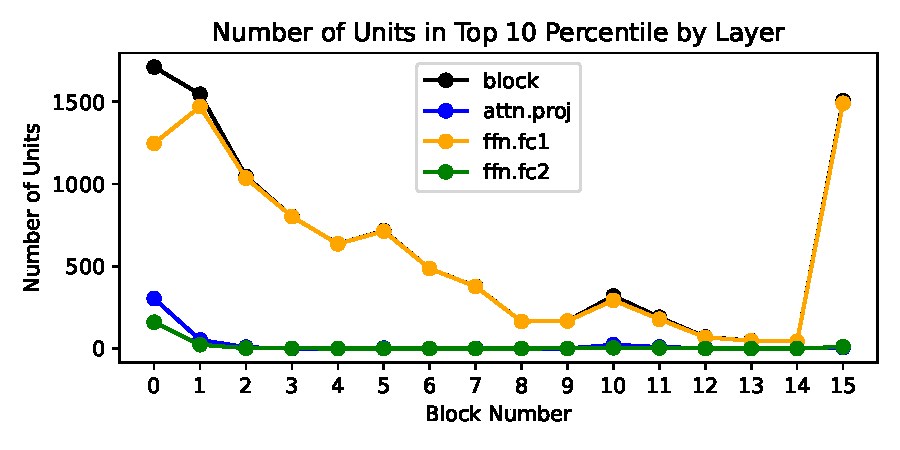
\includegraphics[width=\textwidth]{figures/mem_units_per_layer_num.pdf}
      \caption{Number of highly memorizing units by depth and layer type.}
      \label{fig:mem_units_per_layer_num}
   \end{minipage}\hfill
   \begin{minipage}{0.48\textwidth}
      \centering
      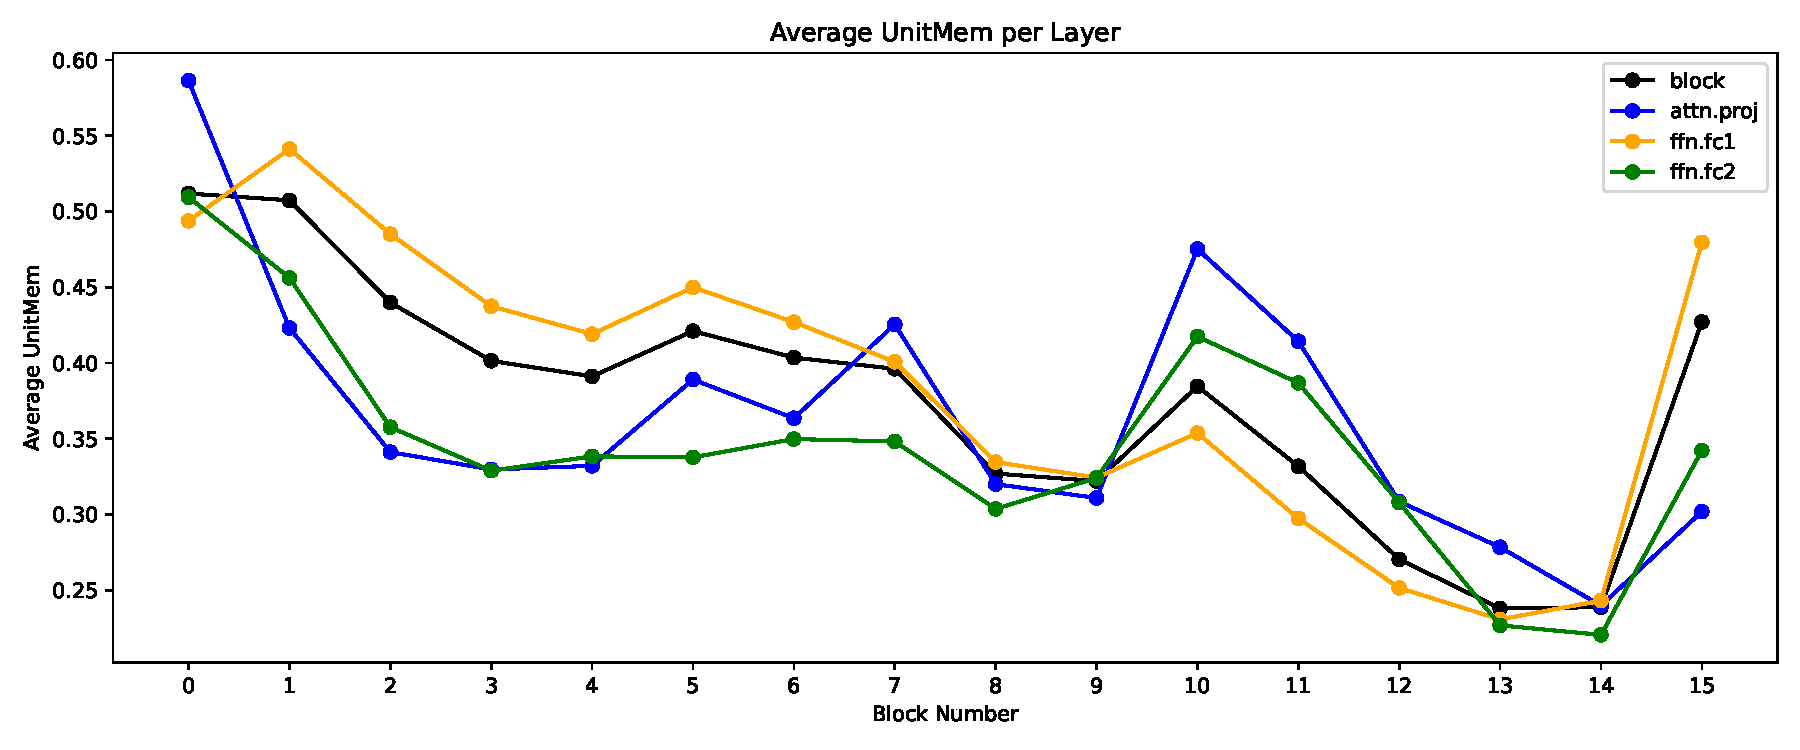
\includegraphics[width=\textwidth]{figures/mem_avg_per_layer_num.pdf}
      \caption{Average UnitMem values by depth and layer type.}
      \label{fig:mem_avg_per_layer_num}
   \end{minipage}
\end{figure}

I also looked at the position \textit{within} a block, i.e., the layer type (\texttt{attn.proj}, \texttt{ffn.fc1}, and \texttt{ffn.fc2}), and noted that the majority of highly memorizing units are located in the \texttt{ffn.fc1} layer, as shown in Figure \ref{fig:mem_units_per_layer_type}.
This trend even holds true when adjusting for the fact that most of the units are located in the \texttt{ffn.fc1} layer (4096 out of 6144 units per block).
When looking at the average \texttt{UnitMem} values per layer type (see Figure~\ref{fig:mem_avg_per_layer_type}), one can see a more even distribution, indicating that \texttt{ffn.fc1} layers also contain a lot of low-memorizing units.
Figure~\ref{fig:mem_max_per_layer_num} shows that the unit with maximal \texttt{UnitMem} value of each block is always found in the \texttt{ffn.fc1} layer.
\begin{figure}[ht]
   \centering
   \begin{minipage}{0.48\textwidth}
      \centering
      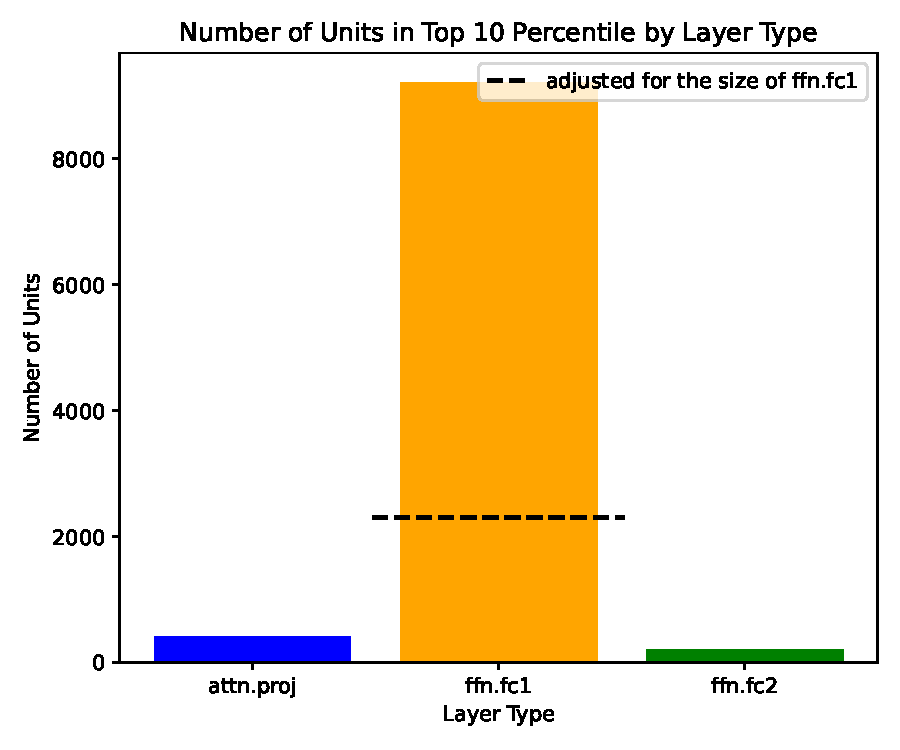
\includegraphics[width=\textwidth]{figures/mem_units_per_layer_type.pdf}
      \caption{Number of highly memorizing units per layer type.}
      \label{fig:mem_units_per_layer_type}
   \end{minipage}\hfill
   \begin{minipage}{0.48\textwidth}
      \centering
      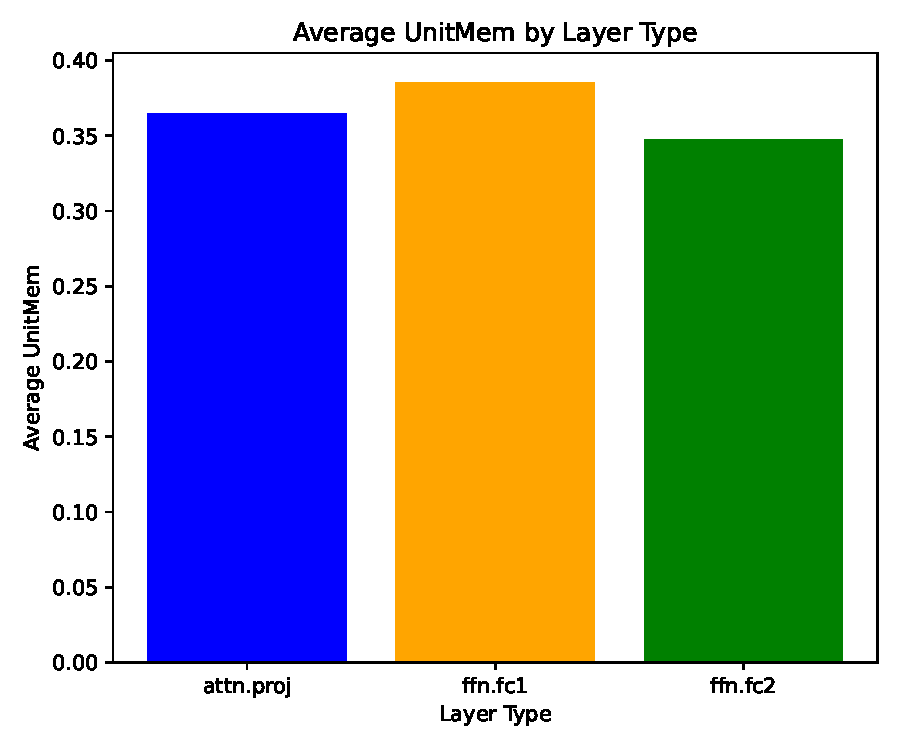
\includegraphics[width=\textwidth]{figures/mem_avg_per_layer_type.pdf}
      \caption{Average UnitMem values per layer type.}
      \label{fig:mem_avg_per_layer_type}
   \end{minipage}
\end{figure}

\begin{figure}[ht]
   \centering
   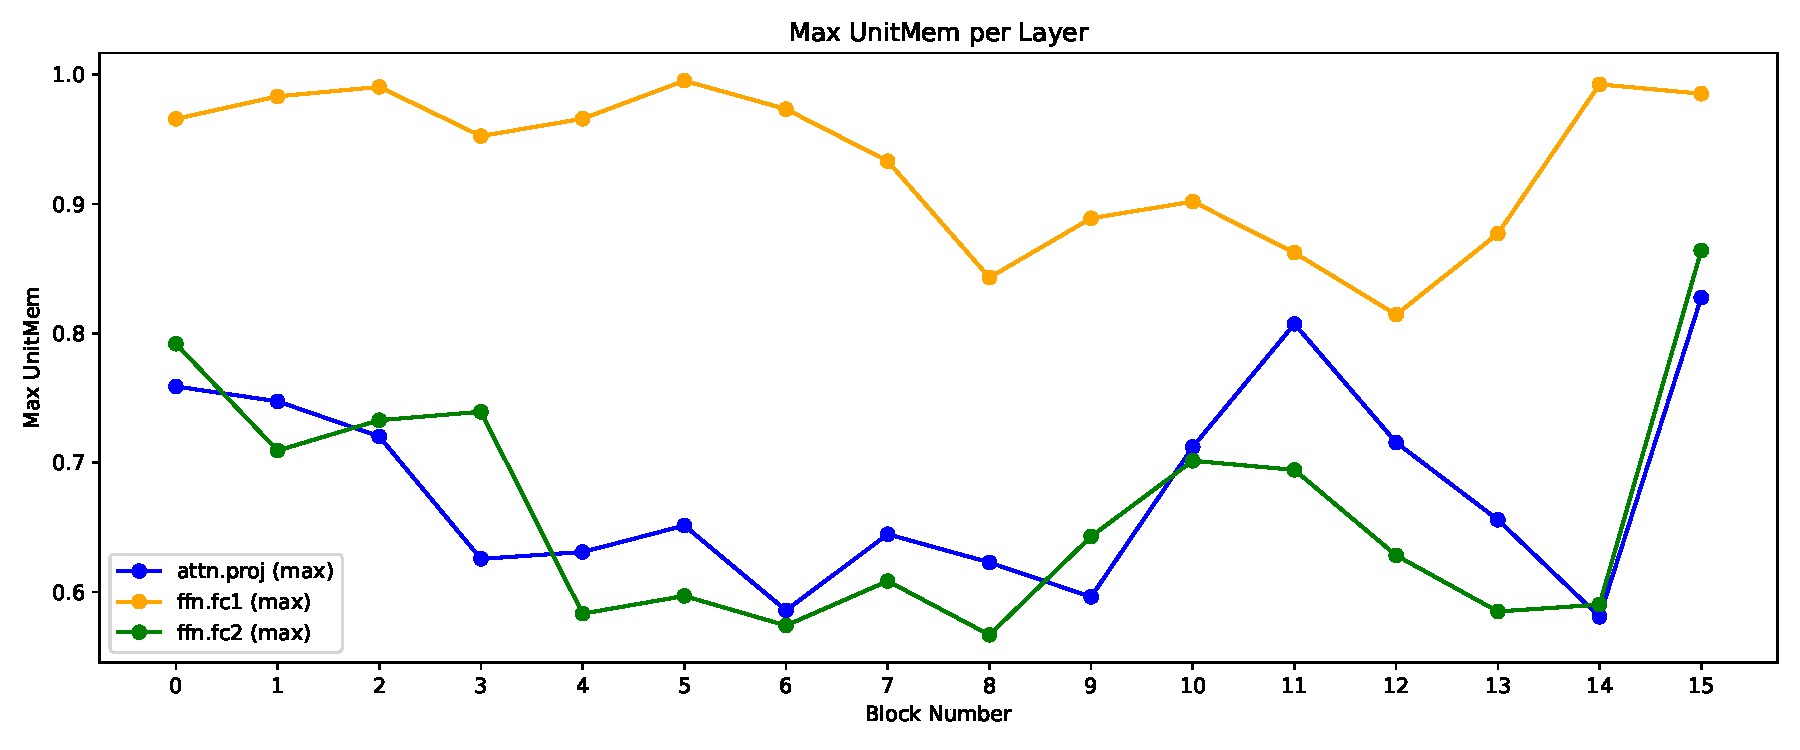
\includegraphics[width=0.7\textwidth]{figures/mem_max_per_layer_num.pdf}
   \caption{Maximum \texttt{UnitMem} value by depth and layer type.}
   \label{fig:mem_max_per_layer_num}
\end{figure}

\subsection{Memorized Samples}
My experiments showed that only a relatively small number of samples are responsible for the high \texttt{UnitMem} values of the units in $\mathcal{U}_{10}$.
Only about 27.2\% of the samples in $\mathcal{D}^\prime$ are responsible for the maximal activation of at least one unit in $\mathcal{U}_{10}$ (i.e., have a \texttt{NumMemUnits} value greater than 0).
At the same time, already 1\% of the samples in $\mathcal{D}^\prime$ are responsible for the maximal activation of 49\% of the units in $\mathcal{U}_{10}$.
10\% of the samples in $\mathcal{D}^\prime$ are responsible for the maximal activation of 83\% of the units in $\mathcal{U}_{10}$.
\footnote{Additionally, undocumented experiments suggested that the portion of memorized samples may be even smaller when looking at a larger dataset $\mathcal{D}^\prime$.}

I also looked at the samples that maximally activate the highest number of highly memorizing units, i.e., the samples with the highest \texttt{NumMemUnits} value, and performed a qualitative assessment.
I found that a large portion of these samples show a spatially repeating high-frequency pattern or huge areas of constant color (see Figure \ref{fig:mem_samples}).

To examine how the memorized samples differ depending on the block depth, I looked at the samples that maximally activate the top 10 units (in terms of \texttt{UnitMem} value) in the \texttt{ffn.fc1} layer of blocks 0, 5, 10, and 15.
While the samples for blocks 0 and 5 are quite diverse, in block 10, 7 out of 10 samples stem from the same class, and in block 15, all top 10 \texttt{UnitMem} scores originate from the same image, as can be seen in Figure~\ref{fig:mem_samples_per_layer}.

\section{Future Work}
\begin{enumerate}
   \item The last observation (less diversity in memorized samples with increasing depth) is very interesting and should be further investigated in a quantitative manner.
   The per-class as well as the per-image distribution are interesting aspects to look at.
   \item The same experiments should be performed on different model depths.
   \item The influence of the class on memorization may be interesting to explore.
   \item Other relevant layers like \texttt{head} may also be interesting to look at.
   \item The findings in~\ref{look_at_val} are unexpected and should be further investigated/thought about (they may not even be correct).
\end{enumerate}



\bibliography{iclr2025_conference}
\bibliographystyle{iclr2025_conference}

\newpage
\appendix
\section{Appendix}
\subsection{A Look at the Validation Set}\label{look_at_val}\footnote{This section is not yet fully verified.}
For sanity check, I constructed a dataset $\mathcal{D}_{val}$ of 256 images per class for the same 32 classes as above from the ImageNet-1k validation set.
I used the data set $\mathcal{D}_{all} = \mathcal{D}_{val} \cup \mathcal{D}^\prime$ consisting of 16,384 images to calculate the \texttt{UnitMem} values.

I expected to see less memorization for samples in $\mathcal{D}_{val}$ as the model was not trained on these images.\footnote{maybe it was?}
Figure~\ref{fig:val_respon_num} shows that the number of \texttt{UnitMem} scores caused by samples from the validation set is slightly higher than for samples from the training set.
Restricting the analysis to only the units in $\mathcal{U}_{10,\mathcal{D}_{all}}$ (obtained as in equation~\ref{eq:mem_units} but on $\mathcal{D}_{all}$), I saw that this trend gets stronger.

\begin{figure}[ht]
   \centering
   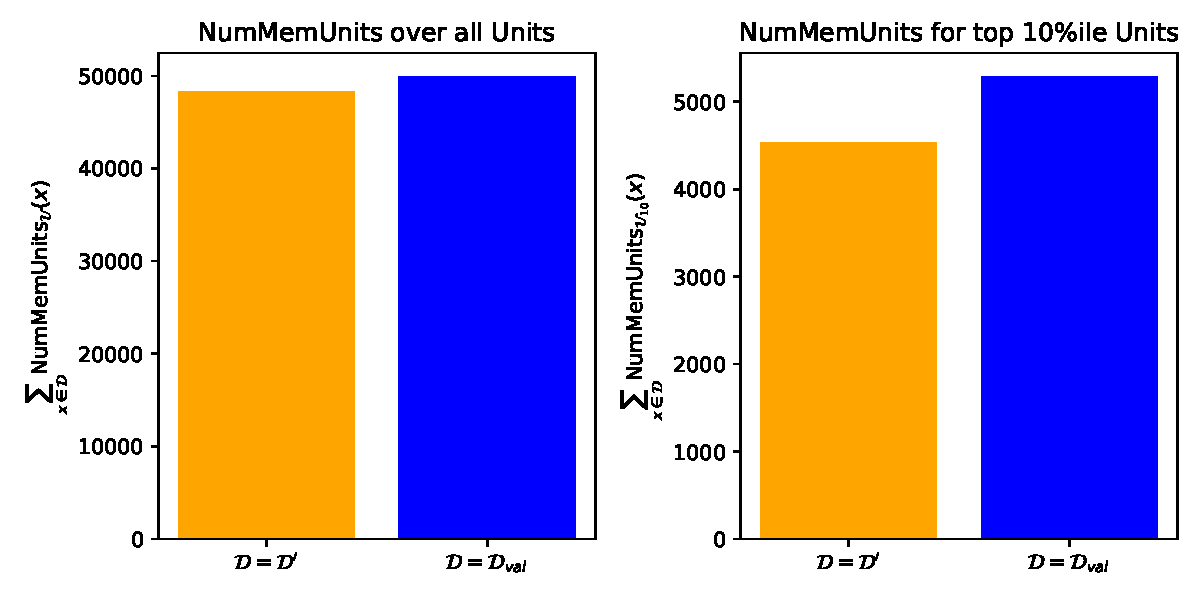
\includegraphics[width=0.7\textwidth]{figures/num_mem_units_train_val.pdf}
   \caption{Number of UnitMem scores caused by samples from the training and validation set.}
   \label{fig:val_respon_num}
\end{figure}
\newpage
\subsection{Memorized Samples}
\begin{figure}[ht]
   \centering
   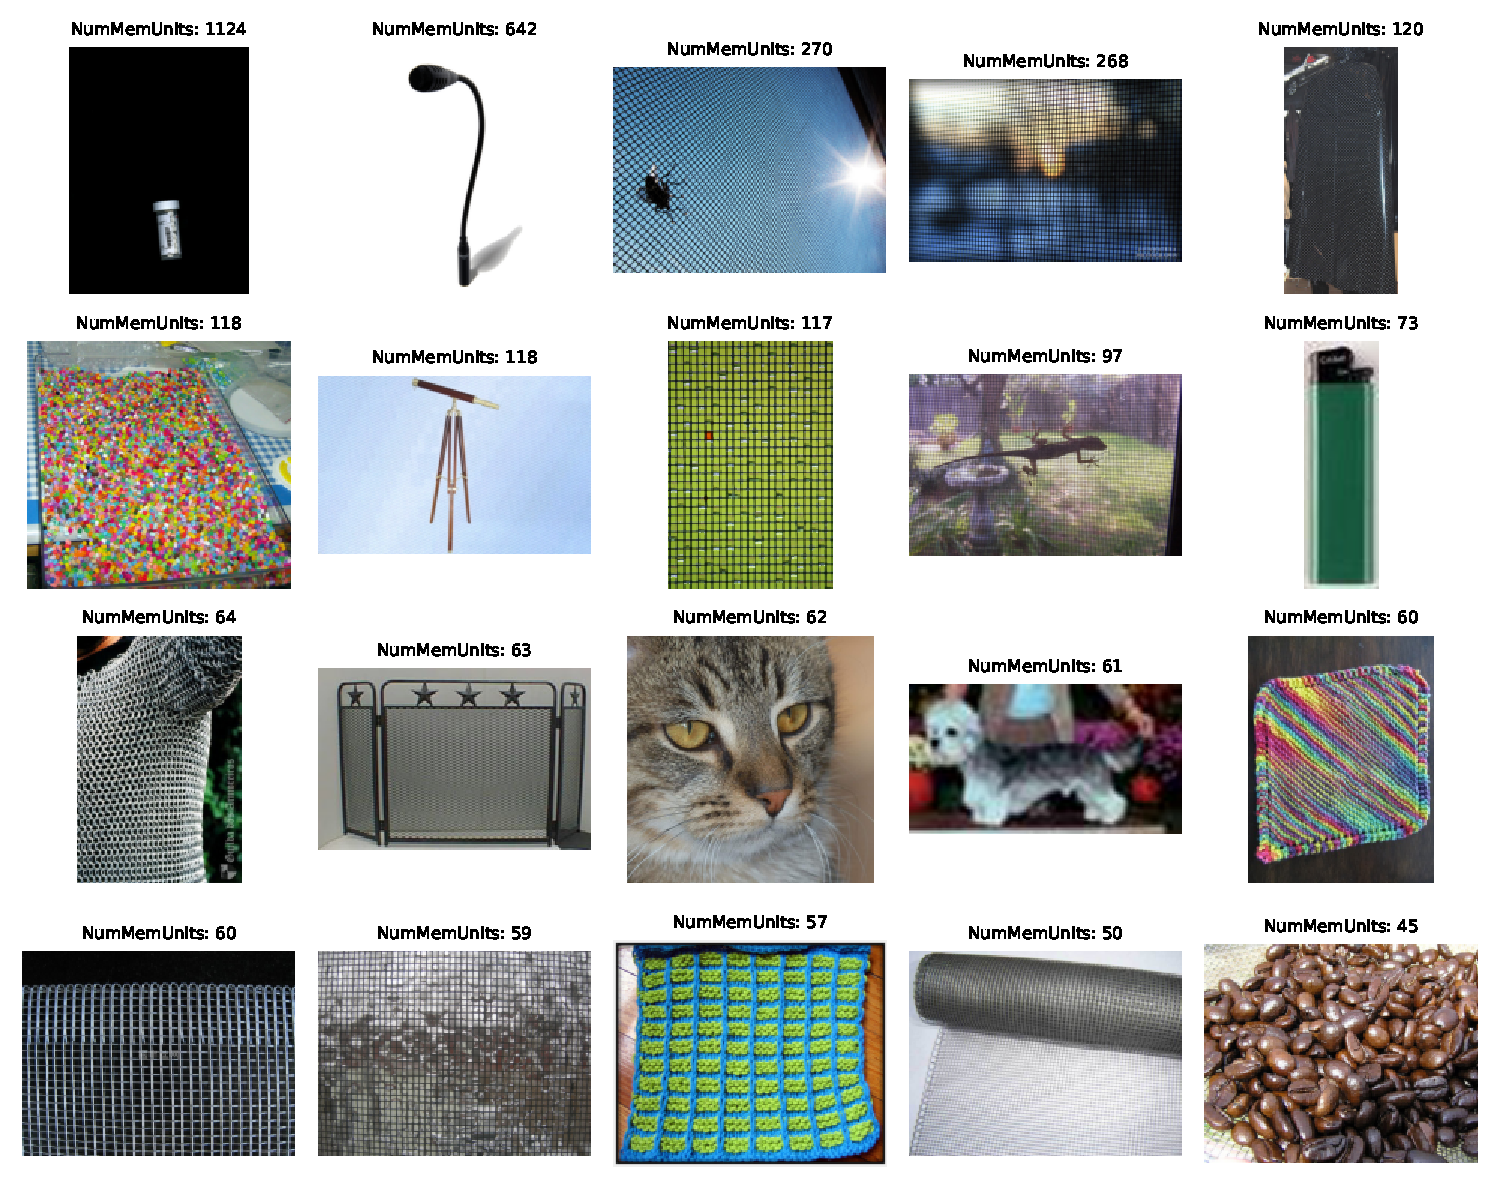
\includegraphics[width=0.9\textwidth]{figures/mem_samples.pdf}
   \caption{Samples that maximally activate the highest number of highly memorizing units.}
   \label{fig:mem_samples}
\end{figure}

\begin{figure}[ht]
   \centering
   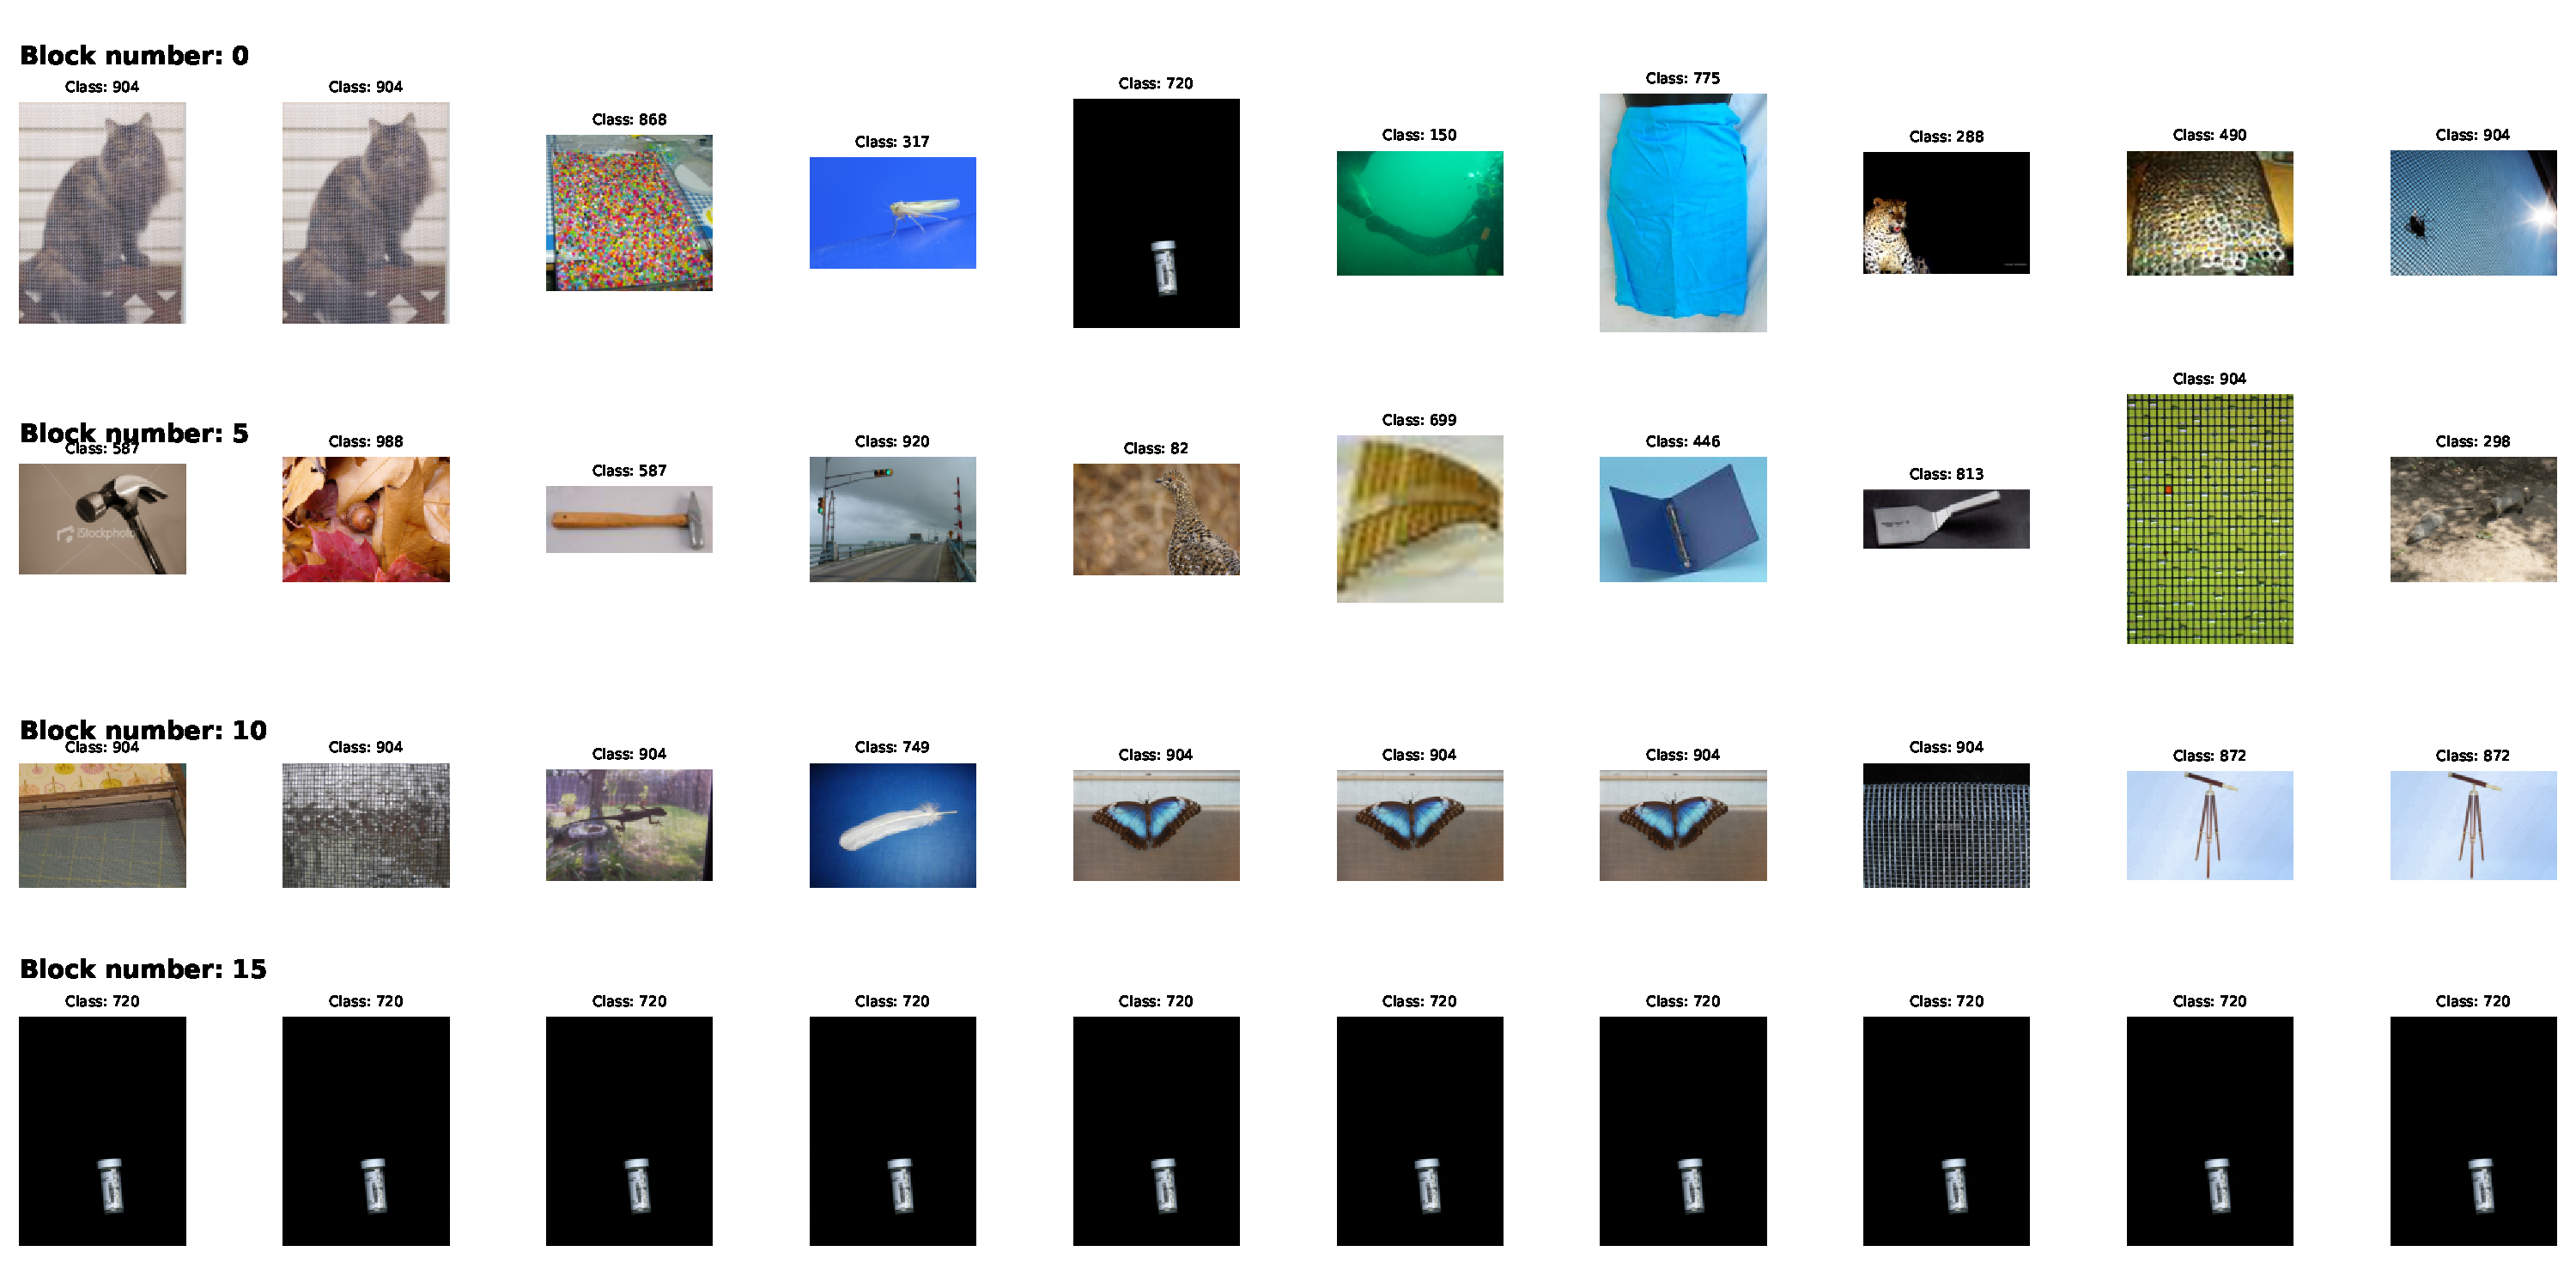
\includegraphics[width=\textwidth]{figures/mem_samples_per_layer.pdf}
   \caption{Samples maximally activating the top 10 units in the ffn.fc1 layer of blocks 0, 5, 10, and 15.}
   \label{fig:mem_samples_per_layer}
\end{figure}


\end{document}
